%draft
\nocite{*}
\documentclass[12pt,a4paper]{article}
\usepackage[left=2.5cm, right=4.5cm, top=2.5cm, bottom=2cm]{geometry}
\usepackage[onehalfspacing]{setspace}
\usepackage[utf8]{inputenc}
\usepackage{ngerman}
\usepackage{bibgerm}
\setlength\parindent{0pt}

\usepackage{graphicx}
\usepackage{subfig}
\usepackage{wrapfig}
\usepackage{caption}

\usepackage{sidecap}
\usepackage{tikz}
\usetikzlibrary{calc}
\usetikzlibrary{shapes,arrows}
\usetikzlibrary{arrows.meta}
\usepackage{environ}
\usepackage{tikz-3dplot}
\usepackage{import}
\usepackage{calc}
\usepackage{pgfmath}
\usepackage{ifthen}
\usepackage{pgfplots}
\usepgfplotslibrary{fillbetween}
\usepackage{amsmath}
\usepackage{makecell}
\usepackage{xr}
\usepackage{xurl}
\usepackage{footnote}
\usepackage[perpage, hang]{footmisc}
\usepackage{tablefootnote}
\usepackage{tabularx}
\usepackage{textcomp}
\usepackage[section]{placeins}
\usepackage{hyperref}
\setlength\footnotemargin{10pt}
\usepackage{listings}
\usepackage{chngcntr}
\usepackage{lipsum}
\usepackage{color, colortbl}
\usepackage{multirow}
\newcommand{\captionref} [1]{\textit{\nameref{#1}}}
\newcolumntype{x}[1]{>{\centering\arraybackslash}p{#1}}

\tikzset{%
  block/.style    = {draw, thick, rectangle, minimum height = 3em,
    minimum width = 3em},
  sum/.style      = {draw, circle, node distance = 1.5cm}, % Adder
  input/.style    = {coordinate}, % Input
  output/.style   = {coordinate}, % Output
   base/.style = {rectangle, rounded corners, draw=black, minimum width=2cm, minimum height=1cm, text centered}
}

\begin{document}
\counterwithin{figure}{section}
\counterwithin{table}{section}
\counterwithin{lstlisting}{section}
\numberwithin{equation}{section}

\author{Philipp Bleimund}

\begin{titlepage}
    \begin{center}
        
\includegraphics[width=7cm]{images/logo.pdf}\\
        \textbf{Evangelisches Gymnasium Werther}\\[8ex]
        \LARGE{\textbf{Besondere Lernleistung}}\\[3ex]
        \huge{\textbf{Prozesse und Threads}}\\[2ex]
        \large{\textbf{anhand einer Rasterbildsoftware}}\\ [50ex]
        \normalsize{}
        \begin{tabular}{ll}
            Verfasser:            & \quad \textbf{Philipp Bleimund}     \\[3ex]
            Kurs:                 & \quad Grundkurs Informatik          \\ [1ex]
            Betreuende Lehrkraft: & \quad Herr Christian Möllenbrock    \\[1ex]
            Abgabetermin:         & \quad 07.04.2022                       \\[1ex]
        \end{tabular}
    \end{center}
\end{titlepage}
\setcounter{page}{2}
\newpage

\tableofcontents
\thispagestyle{empty}
\clearpage
\newpage

%Einleitung
\section{Programm}
Um die Methoden der Threads in einer Realen Situation zu nutzen, habe ich mich entschlossen ein Programm, welches stark von Threads profitieren kann, zu programmieren.  

Ich habe mich für ein Programm eintscheiden, mit dem man ein Bild mit vielen weiteren Bildern rekrieren kann. Es wird demnach ein Mosaik aus Bildern erstellt.

\begin{figure}[h]
    \centering
    \subfloat[\centering Input]{
        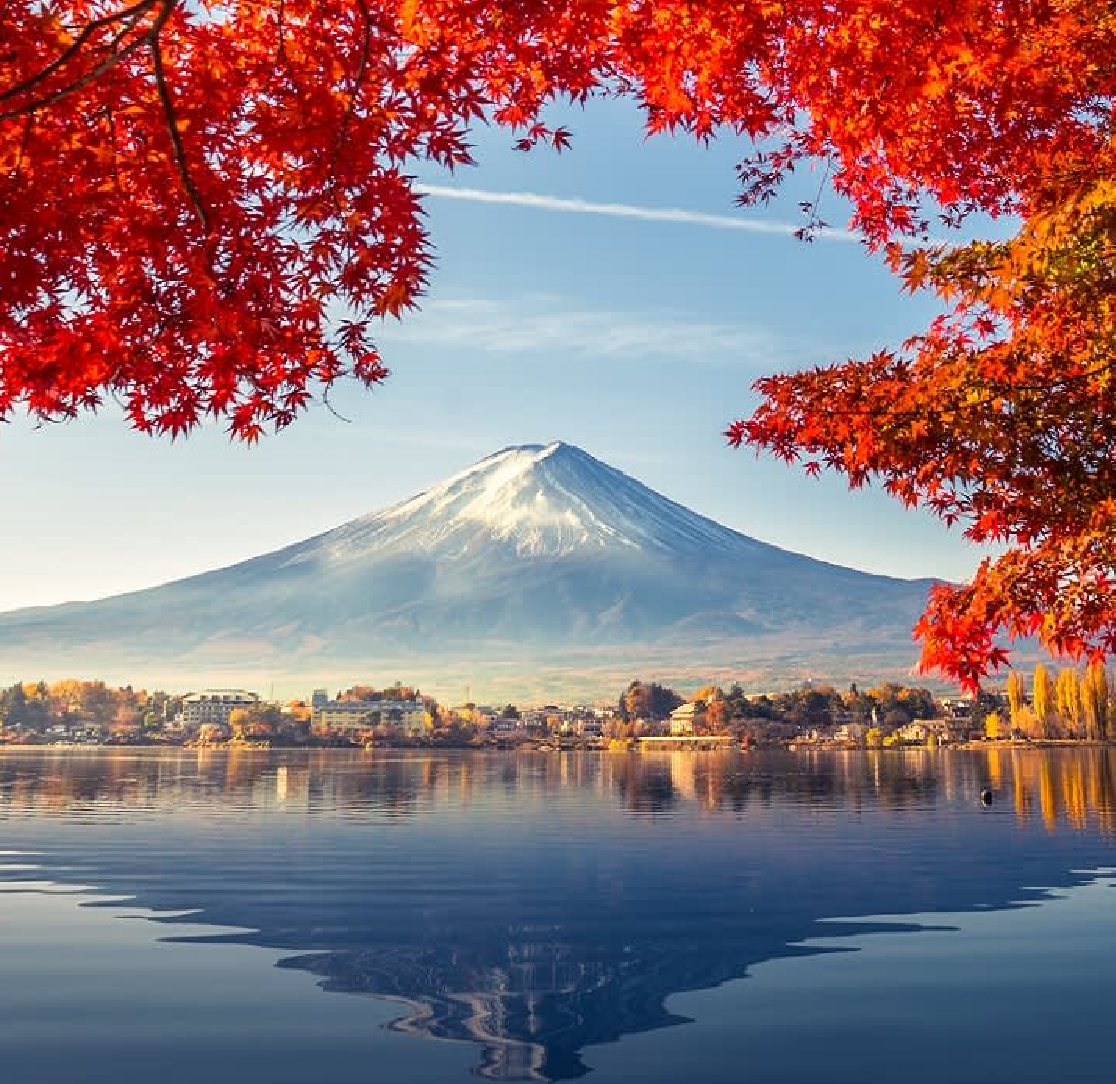
\includegraphics[height=5cm]{images/Source_100x100.pdf}
    }
    \subfloat[\centering Output]{
        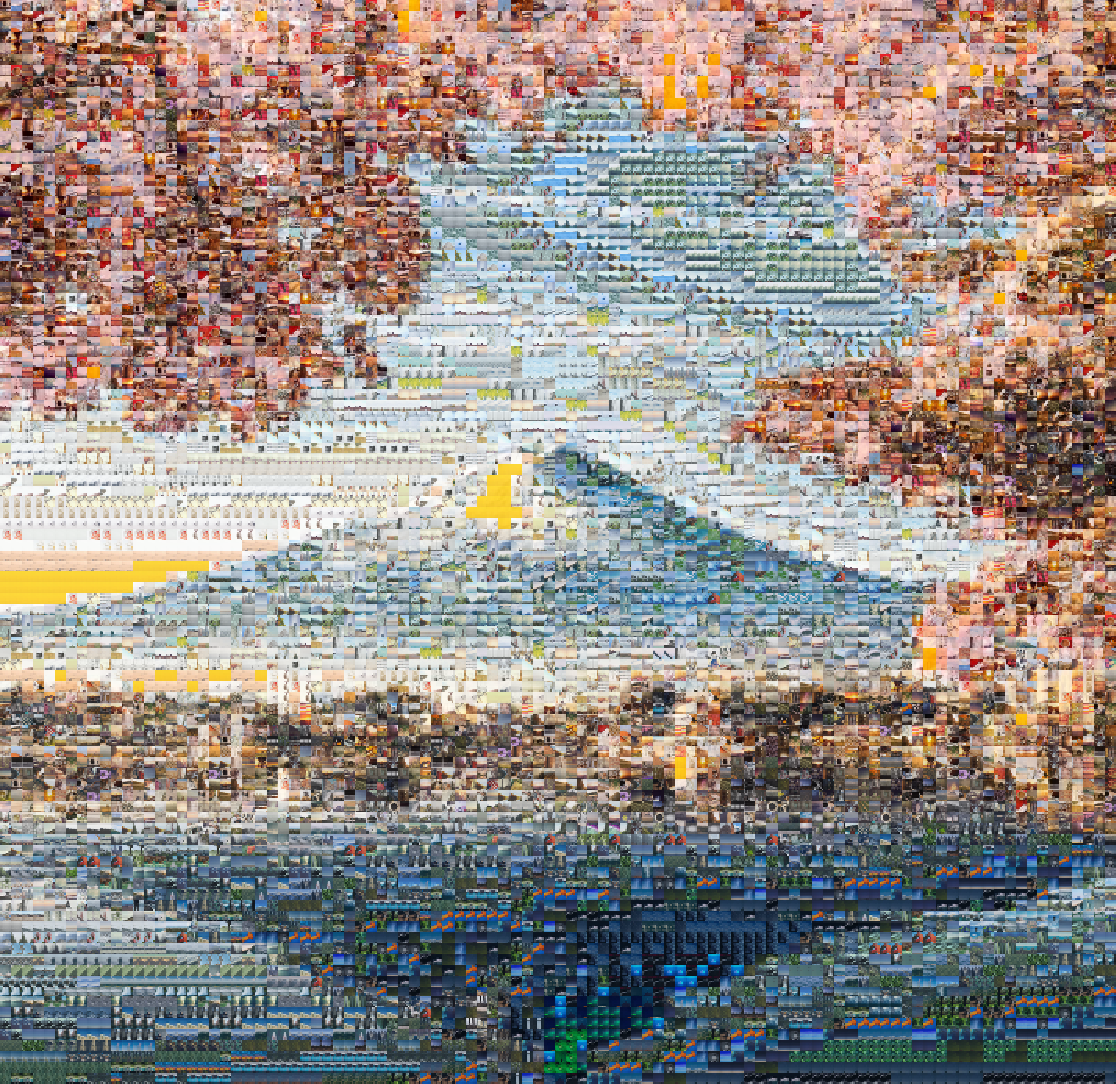
\includegraphics[height=5cm]{images/Render_100x100.pdf}
    }
    \caption[Programm Funktion]{Funktionsweise des Programmes}
\end{figure}

Die anwendung von Threads kommt in dem Programm in vielen Stellen vor. Im folgen werde ich mich auf den Algorythmus der Bild analyse und verarbeitung beziehen. Andere aspekte, wie die implementation des Testmodus und andere Features, die in der App vorhanden sind, werden kurz im Anhang erwähnt.
\newpage

%Threads
\section{Threads und Prozesse}

\subsection{Einleitung}
Prozesse sind die Ausführung eines Programms auf dem Prozessor. Jedoch kann ein Prozessor maximal ein Prozess gleichzeitig ausführen. Um Verwirrung zu beseitigen möchte ich darauf hinweisen, dass selbst moderne Prozessoren nicht in der Lage sind mehrere Prozesse auszuführen. Diese ``Illusion'' wird erzeugt, da ein Prozessor(Bauteil) mehre Kerne hat. Diese Kerne sind die eigentlichen Prozessoren. In Zukunft werde ich den Begriff Kerne nutzen um die Unterscheidung zu erleichtern. Um trotzdem mehrere Prozesse gleichzeitig zu bearbeiten, werden den einzelnen Kernen die Prozesse für nur wenige Millisekunden zugeordnet. Diese nennt man auch Virtuelle Threads. Jeder Virtuelle Thread kann einem realem Kern zugeordnet werden. Jedoch wird nicht jeder Process gleich lange einem Kern zugeordnet. Die Prozesse konkurrieren um ihre Zeit. Denn schließlich soll mein Computerspiel nicht die gleiche Zeit bekommen, wie meine Stoppuhr app. Diese wechsel zwischen den einzelnen Prozessen nennt man auch Kontextwechsel. Der Kontext des Kerns ändert sich demnach.

\begin{figure}[h]
    \centering
    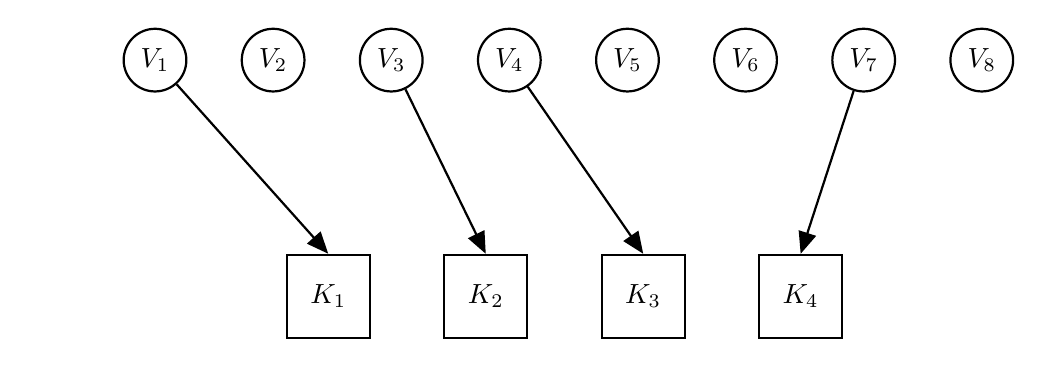
\begin{tikzpicture}[auto, thick, node distance=2cm, >=triangle 45]
        \draw
        node at(0,0)[name=start1]{}
        node [sum, name=VThread1, right of=start1]{$V_1$}
        node [sum, name=VThread2, right of=VThread1]{$V_2$}
        node [sum, name=VThread3, right of=VThread2]{$V_3$}
        node [sum, name=VThread4, right of=VThread3]{$V_4$}
        node [sum, name=VThread5, right of=VThread4]{$V_5$}
        node [sum, name=VThread6, right of=VThread5]{$V_6$}
        node [sum, name=VThread7, right of=VThread6]{$V_7$}
        node [sum, name=VThread8, right of=VThread7]{$V_8$};
        \draw
        node at(1.7,-3)[name=start2]{}
        node [block, name=Kern1, right of=start2]{$K_1$}
        node [block, name=Kern2, right of=Kern1]{$K_2$}
        node [block, name=Kern3, right of=Kern2]{$K_3$}
        node [block, name=Kern4, right of=Kern3]{$K_4$};
        \draw[->](VThread1) -- node{} (Kern1.north);
        \draw[->](VThread3) -- node{} (Kern2.north);
        \draw[->](VThread4) -- node{} (Kern3.north);
        \draw[->](VThread7) -- node{} (Kern4.north);
    \end{tikzpicture}
    \caption{Aufteilung von Virtuellen Threads auf Kernel}
\end{figure}

\subsection{Aufbau von Prozessen}

Prozesse müssen jedoch noch ein wenig mehr als nur ein Stück code besitzen, um aktiv zu werden. Generell kann man sagen, dass Prozesse aus 7 Elementen bestehen.
Diese nennt man Prozesskontext. Innerhalb des Prozesskontextes gibt es noch den Hardwarekontext.
\begin{itemize}
    \setlength\itemsep{0pt}
    \item Das auszuführende Programm
    \item Die Daten des Programmes. Umfasst etwa die Globalen variablen.
    \item Einen Stack. Ein Stack funktioniert nach dem push und pop verfahren und speichert die lokalen Variablen für einen schnelleren zugriff.
    \item Kernelstack. Umfasst die Systemaufrufe des Prozesses.
          \begin{itemize}
              \item CPU Register. Kann in den meisten Fällen nur ein Befehl speichern (64bit Prozessor = 64bits im Register)
              \item MMU Register, dass den zugriff auf den Arbeitsspeicher verwaltet.
          \end{itemize}
\end{itemize}

Da ein Prozess viele Kontextwechsel durchleben wird, muss das Betriebssystem bestimmte Register speichern. Dazu gehört aus dem Hardwarekontext:

\begin{itemize}
    \setlength\itemsep{0pt}
    \item Instruction Pointer - Die Speicheradresse des nächsten Befehls.
    \item Instruction Register - Der aktuelle Befehl.
    \item Stackpointer - Speichert das ende des Stacks.
    \item Basepointer - Speicheradresse des aktuellen Elementes im Stack.
    \item Akkumulator - Speichert, Ergebnisse der ALU
\end{itemize}

Dies sind die wichtigsten Informationen, um die Rechenoperationen weiterführen zu können. Das Betriebssystem braucht jedoch noch weitere Informationen über einen Prozess. Diese werden auch Systemkontext genannt. Die wichtigsten davon sind:

\begin{itemize}
    \setlength\itemsep{0pt}
    \item Ort in der Prozesstabelle
    \item PID - Prozessnummer
    \item Prozesszustand
    \item Priorität
    \item Eltern- oder Kindprozesse
    \item Zugriffsrechte - Linux: -20 bis 19; Windows: Rechte werden einzeln zugeteilt
    \item Erlaubte Ressourcenmengen - Bsp. Maximaler RAM verbrauch
    \item Verwendete Dateien - Um zu verhindern, dass mehre Prozesse an einer Datei arbeiten
    \item Zugeordnete Geräte - Maus, Tastatur, ...
\end{itemize}

Mithilfe der Prozesstabelle kann das Betriebssystem die einzelnen Prozesse speichern. In dieser werden Prozesskontrollblöcke gespeichert, welche den Hardwarekontext und Systemkontext beinhaltet. Bei einem Kontextwechsel wird der Prozesskontext aus der Prozesstabelle wieder hergestellt.

\newpage

\subsection{Verwalten der Prozesse}

Jedes Betriebssystem muss einen weg haben, um effektiv die Kontextwechsel der Prozesse durchführen zu können. Dazu wird in den meisten Fällen ein \captionref{Warteschlange Prozesse} verwendet. Auch hat ein Prozess deutlich mehr Zustände als nur \textit{untätig} und \textit{rechnend} in einem modernen Betriebssystem. Dazu wird heutzutage meistens das \captionref{Prozessmodell} oder eine modifizierte Variante. Linux als Beispiel verwendet ein \textit{8-Zustands Prozessmodell}, welches das Modell mit einem \textit{kernel rechnend} Zustand erweitert.

\begin{figure}[h]
    \centering
    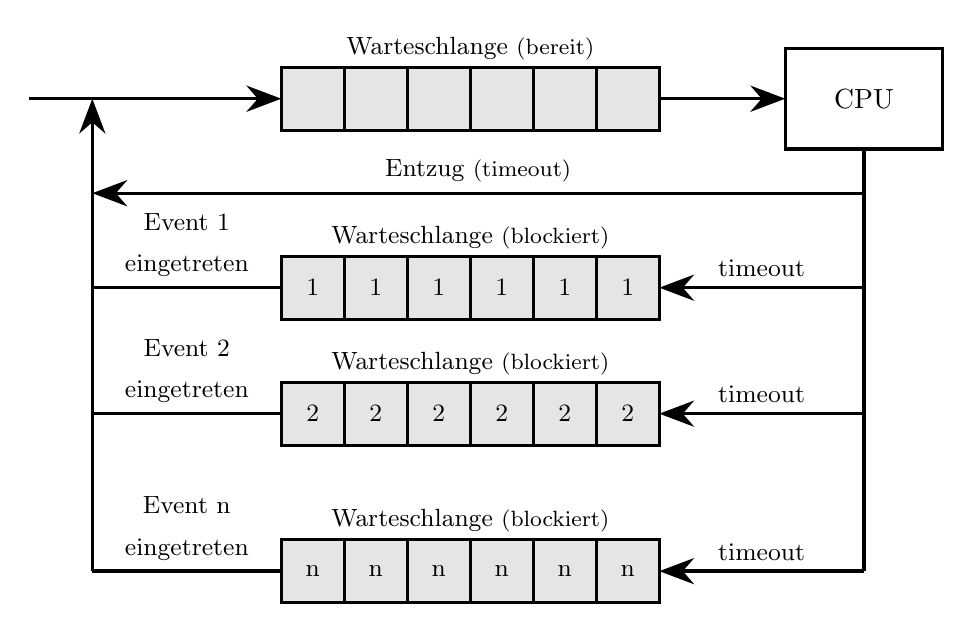
\begin{tikzpicture}[y=-1cm, scale=0.8]
    \pgfmathsetmacro\start{2}
    \pgfmathsetmacro\endValue{5}
    \draw[very thick, -{Stealth[scale=1.5]}](-2,1.5) -- (\start,1.5);

    %Warteschlange
    \foreach \x in {0,...,\endValue}{
        \filldraw[very thick, draw = black, fill = black!10](\start+\x, 1) rectangle (\start+\x+1, 2);
    }

    \pgfmathsetmacro\middleLine{\start+((\endValue+1)/2)}
    \node[align=center] at (\middleLine, 0.7){\small Warteschlange \footnotesize(bereit)};

    \draw[very thick, -{Stealth[scale=1.5]}](\start+\endValue+1,1.5) -- (\start+\endValue+3,1.5);

    \draw[very thick, draw = black](\start+\endValue+3, 0.7) rectangle (\start+\endValue+3+2.5, 2.3) node[pos=.5] {CPU};

    %Linien
    \pgfmathsetmacro\middleCPU{\start+\endValue+3+1.25}
    \pgfmathsetmacro\endLine{\start+\endValue+1}

    \draw[very thick](\middleCPU, 2.3) -- (\middleCPU, 9);
    \draw[very thick, -{Stealth[scale=1.5]}](-1, 9) -- (-1, 1.5);

    %Entzug der CPU
    \draw[very thick, -{Stealth[scale=1.5]}](\middleCPU, 3) -- (-1, 3) node [midway, above] {\small Entzug \footnotesize (timeout)};

    %Event 1
    \draw[very thick, -{Stealth[scale=1.5]}](\middleCPU, 4.5) -- (\endLine, 4.5) node [midway, above] {\small timeout};
    \foreach \x in {0,...,\endValue}{
        \filldraw[very thick, draw = black, fill = black!10](\start+\x, 4) rectangle (\start+\x+1, 5) node[pos=.5] {\small 1};
    }
    \node[align=center] at (\middleLine, 3.7){\small Warteschlange \footnotesize(blockiert)};
    \draw[very thick](\start, 4.5) -- (-1, 4.5) node [midway, above, align=center] {\small Event 1\\\small eingetreten};

    %Event 2
    \draw[very thick, -{Stealth[scale=1.5]}](\middleCPU, 6.5) -- (\endLine, 6.5) node [midway, above] {\small timeout};
    \foreach \x in {0,...,\endValue}{
        \filldraw[very thick, draw = black, fill = black!10](\start+\x, 6) rectangle (\start+\x+1, 7) node[pos=.5] {\small 2};
    }
    \node[align=center] at (\middleLine, 5.7){\small Warteschlange \footnotesize(blockiert)};
    \draw[very thick](\start, 6.5) -- (-1, 6.5) node [midway, above, align=center] {\small Event 2\\\small eingetreten};

    %Event n
    \draw[very thick, -{Stealth[scale=1.5]}](\middleCPU, 9) -- (\endLine, 9) node [midway, above] {\small timeout};
    \foreach \x in {0,...,\endValue}{
        \filldraw[very thick, draw = black, fill = black!10](\start+\x, 8.5) rectangle (\start+\x+1, 9.5) node[pos=.5] {\small n};
    }
    \node[align=center] at (\middleLine, 8.2){\small Warteschlange \footnotesize(blockiert)};
    \draw[very thick](\start, 9) -- (-1, 9) node [midway, above, align=center] {\small Event n\\\small eingetreten};
\end{tikzpicture}
    \caption{Warteschlangen System}
    \label{Warteschlange Prozesse}
\end{figure}

\begin{figure}[h]
    \centering
    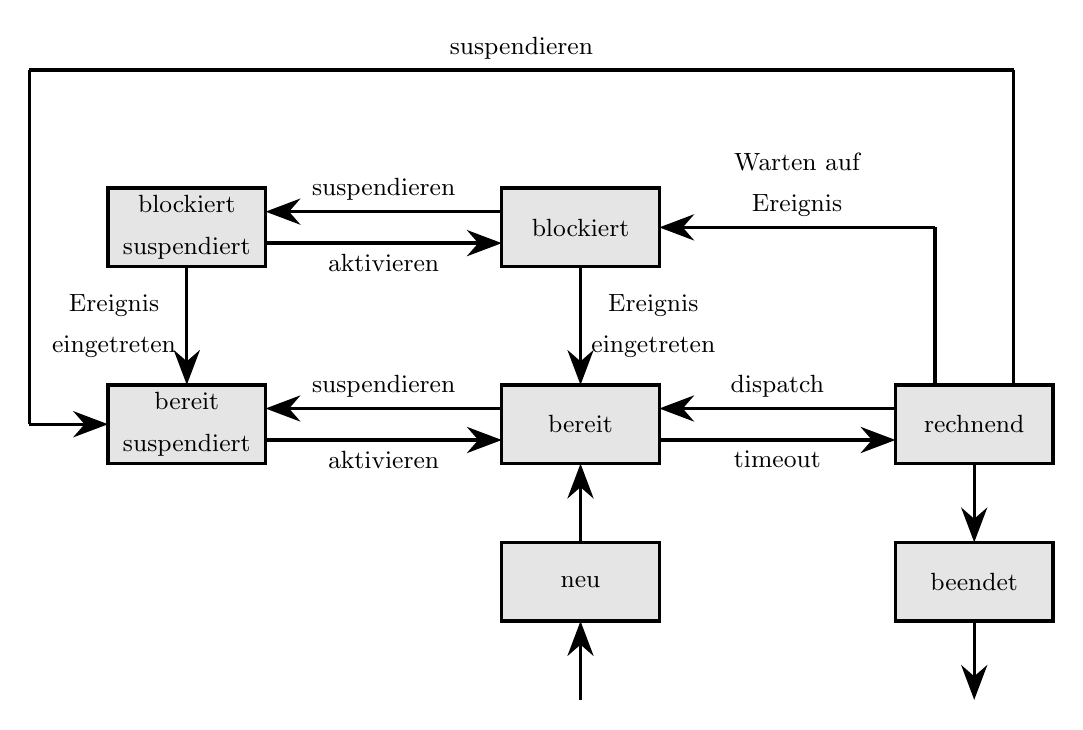
\begin{tikzpicture}
    %neu
    \draw[very thick, -{Stealth[scale=1.5]}](7, 1) -- (7, 2);
    \filldraw[very thick, draw = black, fill = black!10](6, 3) rectangle (8, 2) node[pos=.5] {\small neu};

    %bereit
    \draw[very thick, -{Stealth[scale=1.5]}](7, 3) -- (7, 4);
    \filldraw[very thick, draw = black, fill = black!10](6, 5) rectangle (8, 4) node[pos=.5] {\small bereit};
    \draw[very thick, -{Stealth[scale=1.5]}](8, 4.3) -- (11, 4.3) node [midway, below] {\small timeout};
    \draw[very thick, -{Stealth[scale=1.5]}](6, 4.7) -- (3, 4.7) node [midway, above] {\small suspendieren};

    %blockiert
    \draw[very thick, -{Stealth[scale=1.5]}](7, 6.5) -- (7, 5) node [midway, anchor=west, align=center] {\small Ereignis\\\small eingetreten};
    \filldraw[very thick, draw = black, fill = black!10](6, 7.5) rectangle (8, 6.5) node[pos=.5] {\small blockiert};
    \draw[very thick, -{Stealth[scale=1.5]}](6, 7.2) -- (3, 7.2) node [midway, above] {\small suspendieren};
    
    %beendet
    \filldraw[very thick, draw = black, fill = black!10](11, 3) rectangle (13, 2) node[pos=.5] {\small beendet};
    \draw[very thick, -{Stealth[scale=1.5]}](12, 2) -- (12, 1);

    %rechnend
    \draw[very thick, -{Stealth[scale=1.5]}](12, 4) -- (12, 3);
    \filldraw[very thick, draw = black, fill = black!10](11, 5) rectangle (13, 4) node[pos=.5] {\small rechnend};
    \draw[very thick, -{Stealth[scale=1.5]}](11, 4.7) -- (8, 4.7) node [midway, above] {\small dispatch};
    \draw[very thick](11.5, 5) -- (11.5, 7);
    \draw[very thick, -{Stealth[scale=1.5]}](11.5, 7) -- (8, 7) node [midway, above, align=center] {\small Warten auf \\\small Ereignis};
    \draw[very thick](12.5, 5) -- (12.5, 9);
    \draw[very thick](12.5, 9) -- (0, 9) node [midway, above] {\small suspendieren};
    \draw[very thick](0, 9) -- (0, 4.5);
    \draw[very thick, -{Stealth[scale=1.5]}](0, 4.5) -- (1, 4.5);

    %bereit suspendiert
    \filldraw[very thick, draw = black, fill = black!10](1, 5) rectangle (3, 4) node[pos=.5, align=center] {\small bereit\\\small suspendiert};
    \draw[very thick, -{Stealth[scale=1.5]}](3, 4.3) -- (6, 4.3) node [midway, below] {\small aktivieren};

    %blockiert suspendiert
    \filldraw[very thick, draw = black, fill = black!10](1, 7.5) rectangle (3, 6.5) node[pos=.5, align=center] {\small blockiert\\\small suspendiert};
    \draw[very thick, -{Stealth[scale=1.5]}](2, 6.5) -- (2, 5) node [midway, anchor=east, align=center] {\small Ereignis\\\small eingetreten};
    \draw[very thick, -{Stealth[scale=1.5]}](3, 6.8) -- (6, 6.8) node [midway, below] {\small aktivieren};
\end{tikzpicture}
    \caption{7-Zustands Prozessmodell}
    \label{Prozessmodell}
\end{figure}

\newpage

Wie in der Einleitung schon angesprochen sind die Zustände \textit{bereit} und \textit{rechnend} die wichtigsten Zustände. Mit diesen alleine könnte ein Betriebssystem funktionieren. Es gäbe dazu dann nur eine Warteschlange, in der sich alle Prozesse des Zustandes \textit{bereit} befinden. Idealer Weise implementiert der \textit{Scheduler}\footnote{Programm zum Managen der Warteschlangen.}  einen Algorithmus, welcher die Priorität der Prozesse berücksichtigt. Wie schon erwähnt muss sich der \textit{Dispatcher}\footnote{Programm zum ausführen der Prozesswechsel.} um noch weitere Zustände kümmern. Diese und ihre Beziehungen sind in Grafik \ref{Prozessmodell} zu finden. Zwei davon währen \textit{neu} und \textit{beendet}. Diese sind für eine größere Flexibilität nützlich. Mit dem \textit{beendet} Zustand, können Informationen nachträglich von einem fertigen Prozess aufgerufen werden. Der Zustand \textit{neu} hat die gemeinsame Funktion mit dem \textit{beendet}-Zustand Ressourcen zu sparen.\newline
Ein Entschiedener Fehler ist es anzunehmen, dass alle Prozesse jederzeit Arbeiten wollen. So könnte ein Programm auf eine Tastatur Eingabe oder andere Ereignisse warten. Um diese Funktionalität bereitstellen zu können gibt es den Zustand \textit{blockiert}. In diesen wechselt ein Prozess nach den berechnen und kann aus diesen sich wieder in die Warteschlange der bereiten Prozesse einordnen. In Grafik \ref{Warteschlange Prozesse} werden unterschiedliche Warteschlangen für unterschiedliche Ereignisse erzeugt. Dieses Vorgehen hat den Vorteil gegenüber einer einzelnen ``blockiert-Warteschlange'', dass häufig genutzte Events wie Tastenanschläge nicht von seltenen Events beeinträchtigt werden.\newline
Da es sehr schnell zu vielen Prozessen kommen kann, wird mit den Zuständen \textit{blockiert suspendiert} und \textit{bereit suspendiert} eine Möglichkeit geschaffen, selten genutzte Prozesse aus dem Arbeitsspeicher in den Massenspeicher\footnote{Spezielle Partitionen auf einer Festplatte. Auch \textit{swap} genannt.} zu verschieben. Wie die Namen schon Implizieren Prozesse in den Zuständen \textit{blockiert} und \textit{bereit} jeweils suspendiert und aktiviert werden. Für zusätzliche Geschwindigkeit, können Prozesse selbst im suspendierten Zustand auf Ereignisse reagieren und von \textit{blockiert suspendiert} in \textit{bereit suspendiert} wechseln. Es gibt demnach ein zweites \captionref{Warteschlange Prozesse} für die suspendierten Prozesse. Dieses beinhaltet keinen zugriff auf die CPU, sondern kann die Prozesse maximal aktivieren und in den Arbeitsspeicher verschieben.

\newpage

\subsubsection{Funktionsweise des Schedulers}
\lipsum

\subsection{Threads}
\lipsum

\subsection{Implementation in java}
\lipsum

\subsubsection{ThreadPool}
\lipsum[3-5]

\subsubsection{Thread sicherheit}
\lipsum[3-5]

\section{Quellen}
MapBild :
SynchronousJFXFileChooser : https://stackoverflow.com/questions/28920758/javafx-filechooser-in-swing
Answer from Sergei Tachenov
\newpage

%Das Programm
\section{Programm}
Um die Methoden der Threads in einer Realen Situation zu nutzen, habe ich mich entschlossen ein Programm, welches stark von Threads profitieren kann, zu programmieren.  

Ich habe mich für ein Programm eintscheiden, mit dem man ein Bild mit vielen weiteren Bildern rekrieren kann. Es wird demnach ein Mosaik aus Bildern erstellt.

\begin{figure}[h]
    \centering
    \subfloat[\centering Input]{
        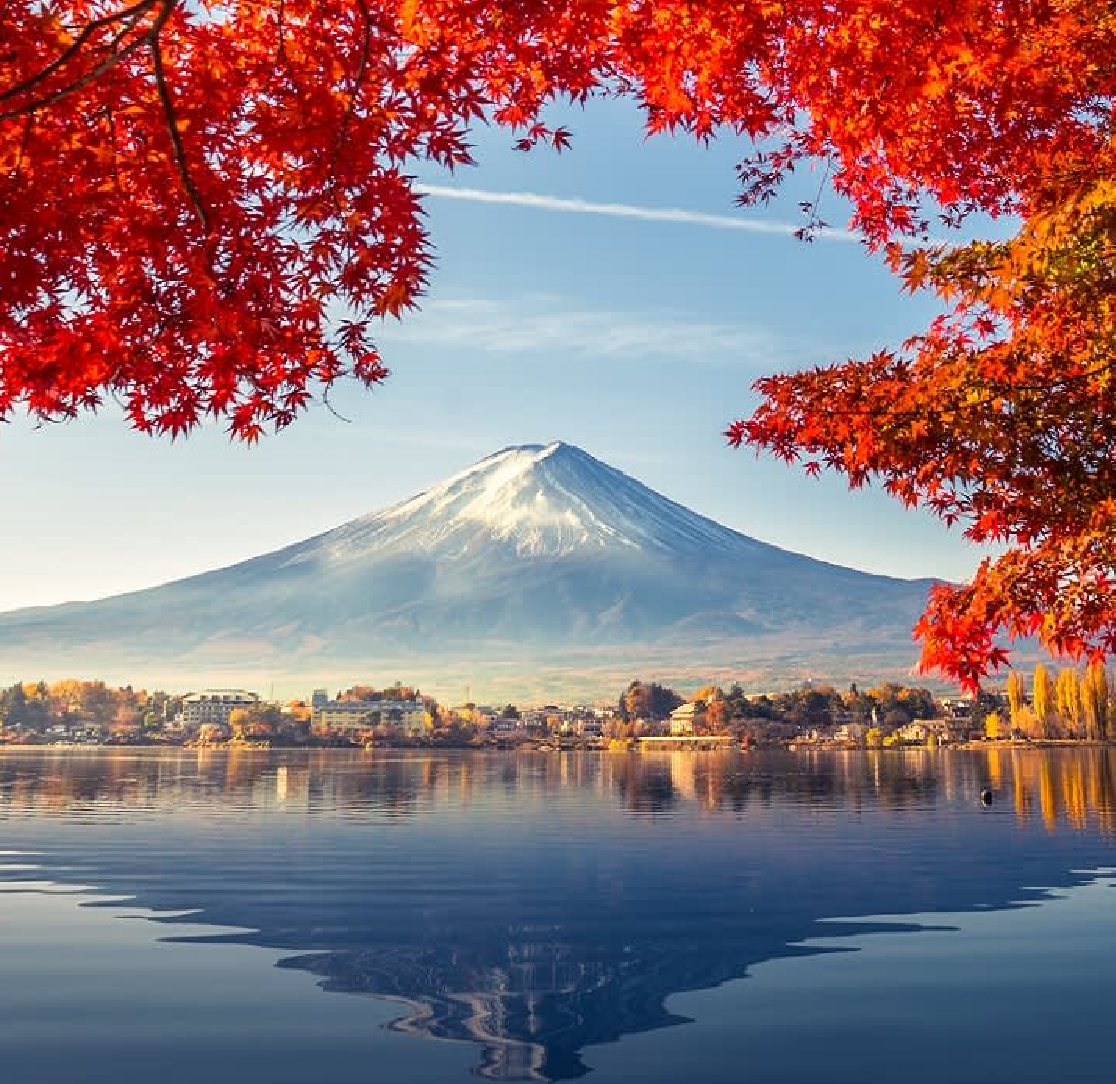
\includegraphics[height=5cm]{images/Source_100x100.pdf}
    }
    \subfloat[\centering Output]{
        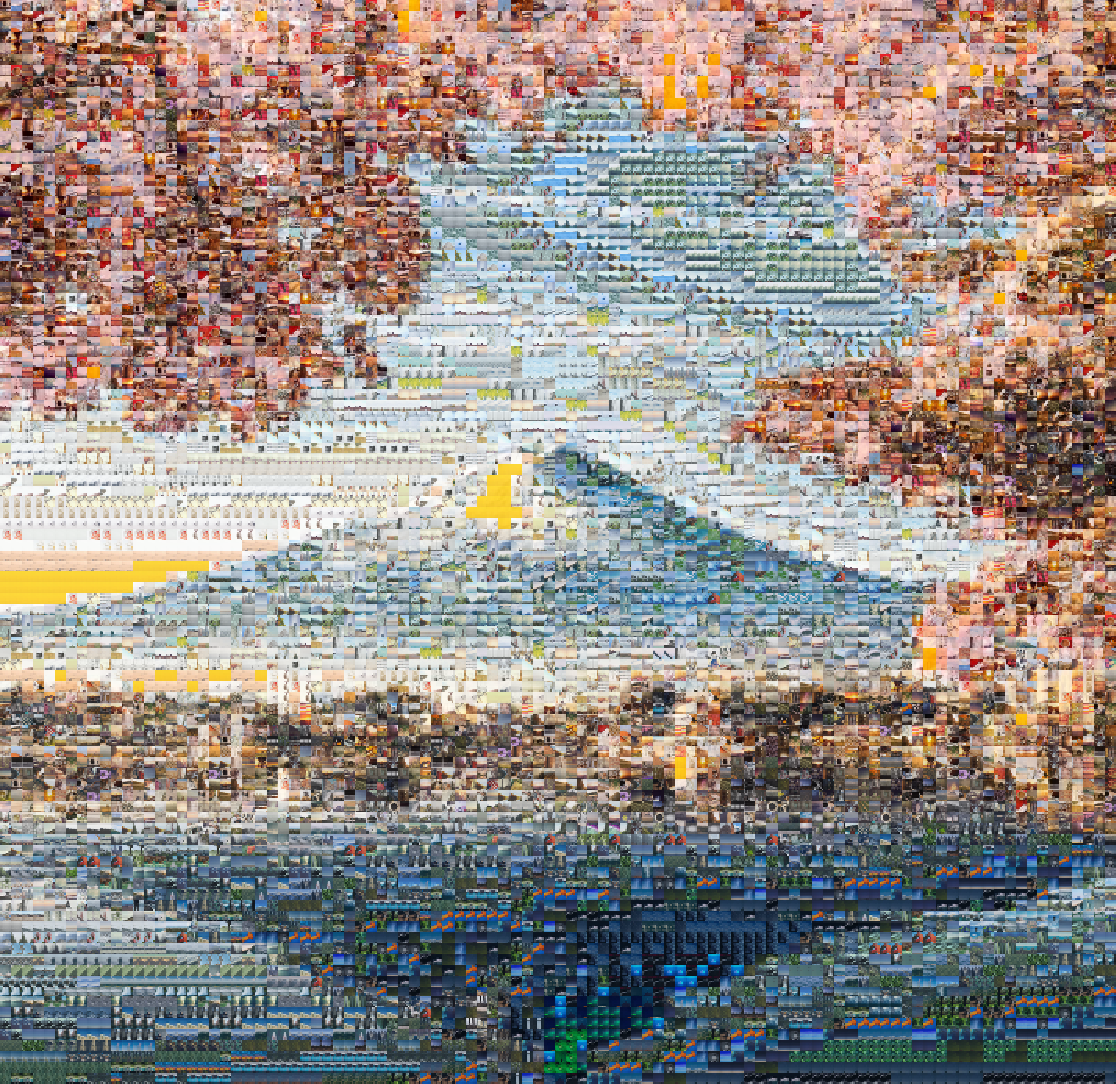
\includegraphics[height=5cm]{images/Render_100x100.pdf}
    }
    \caption[Programm Funktion]{Funktionsweise des Programmes}
\end{figure}

Die anwendung von Threads kommt in dem Programm in vielen Stellen vor. Im folgen werde ich mich auf den Algorythmus der Bild analyse und verarbeitung beziehen. Andere aspekte, wie die implementation des Testmodus und andere Features, die in der App vorhanden sind, werden kurz im Anhang erwähnt.
\newpage
\subsection{Idee}
In der genaueren Betrachtung, muss das Programm das eingegebene Bild vereinfachen. Dies wird durch eine Unterteilung des Bildes in Sektoren erreicht. Die Sektoren sind auch die zukünftigen Stellen für die ausgewählten Bilder. Es wird die durchschnittliche Farbe der Sektoren berechnet. Das selbe vorgehen wird auch auf die ausgewählten Bilder angewendet. Dabei ist ein Bild ein Sektor. Das Vorgehen erlaubt es auch, Datenbanken (im JSON-Format) zu erstellen, da sich die durchschnittliche Farbe der ausgewählten Bilder nicht ändern wird. Anschließend wird mit einem Algorithmus die passenden Bilder für die einzelnen Sektoren berechnet. Dabei unterliegt der Algorithmus der Beschränkung, dass der Nutzer wählen kann, wie häufig ein Bild vorkommen darf. Nach dem Berechnen der benötigten Bilder müssen diese für die Verwendung angepasst werden. Es soll schließlich nicht ein 10x10px großer Teil aus einem 4000x3000px Bild verwendet werden. Dazu wird das Bild erst skaliert und schließlich zurechtgeschnitten. Dabei liegt der Fokus darauf, immer die Mitte des Bildes zu treffen. Das Programm arbeitet schrittweise und die nachfolgenden Kapitel stellen die Reihenfolge dar.
\subsection{Implementation in Java}
\subsubsection{Berechnen der Sektionen}
Das berechnen der Sektionen ist eigentlich ziemlich geradeaus. Die Größe des Bildes ist bekannt und in wie viele Teile dieses aufgeteilt werden soll. Dazu wird zb. die Breite des Bildes mit der vertikalen Anzahl an Sektoren geteilt. Das Problem liegt darin, dass die Breite oder Höhe des Bildes nicht ein redundant von den gewünschten Sektoren ist. Um das Problem anzugehen wird ersterer Schritt nur mit Integers ausgeführt und der Rest berechnet wird. Übergeblieben sind wie viele Spalte auf der X- und Y-Achse gemacht müssen und der Rest der über bleibt. Im nächsten Schritt werden die Größen der Sektoren in Pixeln berechnet. Dies erfolgt dadurch, dass zwei Arrays für die X- und Y-Achse mit der Anzahl an benötigten Spalten gefüllt werden. Ein weiteres Array mit der Anzahl der Spalten wird aufsteigend nummeriert. Das Array wird von einer Methode gemischt. Eine Abschließende Schleife wird mit der Anzahl des Restes wiederholt und bei jedem Schritt wird ein dann zufälliger Wert aus den Array als Index für das Array mit der Größe der Sektoren genutzt. Das nun zufällige Segment wird um 1 erhöht. Die berechneten Werte werden in einem ``splitObj'' gespeichert. In diesem werden die Werte in unterschiedlichsten Arten wie z.B. Koordinaten gespeichert. 

Diese Koordinaten werden im nächsten Schritt benutzt, um ein zweidimensionales Array an \textit{BufferedImages} aus dem Original Bild zu extrahieren. Dazu wird die \textit{getSubimage()} Methode der Klasse \textit{BufferedImage} verwendet.

\subsubsection{Berechnen der durchschnittlichen Farbe}
Das berechnen der durchschnittlichen Farbe von Segmenten und Bildern ist die erste Funktion, welche Threads nutzt. Implementationen von mir, welche Threads benutzen, bestehen meistens aus zwei Klassen. Eine Klasse, welche die Threads erstellt und verwaltet und eine weitere, welche den Code zum berechnen der jeweiligen Anforderung hat. In diesem Falle das Berechnen der durchschnittlichen Farbe. Die Klasse ``computeAverageColor'' besteht aus zwei Methoden. Eine zum Berechnen der Segmente und eine weitere für die gewählten Bilder. Der einzige Unterschied der beiden Methoden ist eine Sicherheitsfunktion in der Methode der Bilder welche wartet, bis genügend RAM verfügbar ist, bevor es das Bild in den RAM läd. Dies ist wichtig, da mehrere Threads gleichzeitig die Bilder im RAM zum Berechnen halten müssen. Je nach RAM Configuration und Bildergröße kann dies zu Komplikationen führen. Um zuverlässig die Größe des Bildes zu berechnen, kann nicht einfach die Dateigröße verwendet werden. Durch Komprimierungsverfahren wie jpg und png kann die Dateigröße eines Bildes um das 10-fache verkleinern. Um die wirkliche Größe zu berechnen, müssen die Dimensionen mal die Farbtiefe gerechnet werden. Die verwendeten BufferedImages haben eine Farbtiefe von 4byte oder 32bit. Um die Dimensionen eines Bildes auszulesen, ohne das gesamte Bild in den Speicher laden zu müssen, wird die ``ImageIO'' Klasse von java genutzt. Die ``ImageIO'' KLasse bietet eine Methode, mit welcher alle ``ImageReader'' eines Bildes erstellt werden. Ein ``ImageReader'' benötigt lediglich die Metadaten eines Bildes, welche nur einen Bruchteil der Dateigröße einsprechen, um die Dimensionen des Bildes zu lesen. Jeder der Threads ruft die Methode ``getAverage()'' der Klasse ``calculateAverage'' auf. Die Methode verlangt ein ``BufferedImage'' und ein enum ``calculateAverage.Method'', welches unterschiedliche Genauigkeitsstufen zum berechnen beinhaltet. Innerhalb der Methode ``getAverage()'' wird erst mit Hilfe des enums ein int definiert, welches beschreibt wie die nachfolgenden for-Schleifen erhöht werden. Weiterhin gibt es dre ``long''. Diese speichern den gesamten rot, blau und grün wert. Anschließend wird das Bild in der vorherigen definierten Schrittgröße durchgegangen und die rot, grün und blau werte des Pixels gespeichert. Zum Schluss wird ein neues ``Color'' Object mit den gesammelten werden geteilt durch die Anzahl der Pixel.

\subsubsection{Erstellen einer Datenbank}
Dieser Schritt wird immer dann durchgeführt, wenn im Programm Bilder ausgewählt wurden, oder eine speicherbare Datenbank erstellt wird. Wenn Datenbanken ausgewählt wurden, wird die eventuell erstellte Datenbank diesen hinzugefügt. Die Klasse ``DatabaseObj'' benötigt zwei Argumente. Eine Liste an Speicherorten der jeweiligen Bilder und ein Array an berechneten durchschnittlichen Farben. Innerhalb des ``DatabaseObj'' werden die beiden Werte der Listen in ``fileAndColor'' Objekten gespeichert. Wie der Name impliziert beinhalten die Objekte den Pfad des Bildes und den dazugehörigen Farbwert. Durch dieses Vorgehen kann ein BinarySort Algorithmus aus das neue Array angewendet werden. dazu hat die ``fileAndColor'' Klasse das ``Comparable'' interface implementiert. Für spätere Verwendung gibt es in den Objekten auch noch einen Zähler, welcher speichert, wie häufig das Bild in der Berechnung verwendet wurde. Alle Variablen der Klasse ``fileAndColor'' sind durch getter- setter-Methoden aufzurufen. Diese habe jedoch die Besonderheit, dass sie das ``synchronized'' Schlüsselwort besitzen (Hyperlink zu Kapitel Threads).
\bigskip
\newline
Besonders werde ich auf die Methode ``compareTo()'', des Interfaces Comparable eingehen. In der Methode werden zwei Farben verglichen. Welche größer und kleiner ist. Die Schwierigkeit liegt darin ein Ergebnis zu bestimmen, wenn vier Werte verglichen werden müssen. Der alpha-Wert, rot-Wert, grün-Wert und blau-Wert. Um ein einfachen und zuverlässigen Vergleich zu machen, nutze ich die Methode ``getRGB()'' der ``Color'' Klasse. Interessant ist jedoch, was diese Methode macht. In der Klasse ``Color'' werden alle vier Werte in einem einzigen Integer gespeichert. Das liegt an der Genauigkeit, womit Farben gemischt werden. Jeder Wert befindet sich in einem Bereich von 0 bis 255. Dies entspricht genau einem Byte. Ein Integer wiederum besteht aus vier Bytes. Die vie Farbwerte werden sozusagen in die vier Bytes des Integers eingesetzt. In der Reihenfolge ``ARGB''.\\
\begin{figure}[h]
    \centering
    \begin{tabular}{c | c | c | c || c}
        alpha(255) & rot(224) & grün(64) & blau(16) & \tikz \definecolor{dkOrange}{rgb} {0.88,0.25,0.06} \fill [dkOrange] (0, 0) rectangle (10pt, 10pt); \\
        \hline
        11111111 & 11100000 & 01000000 & 00010000 & -2080752
    \end{tabular}
\end{figure}
\\Durch dieses Vorgehen wird aus vier Werten ein zuverlässiger Wert erstellt, welcher zum sortieren geeignet ist.

\newpage

\subsubsection{Berechnen der besten Bilder}
Das Berechnen der besten Bilder für die jeweiligen Sektoren wird in der Klasse ``compareColor'' mit der Methode ``compare()'' ausgeführt. Die Methode gibt ein zweidimensionales ``File''-Array zurück. Dies steht dabei für die einzelnen Sektoren. Innerhalb der Methode wird für jeden Sektor ein ``Runnable'' erstellt. (siehe Kapitel Threads). Da es ein Limit für die Verwendung der Bilder gibt, sollen diese gleichmäßig verteilt werden. Um einen solchen Effekt zu erhalten wird eine Liste an ``Runnables'' erstellt und gemischt.

\begin{figure}[h]
    \centering
    \subfloat[\centering ohne mischung]{
        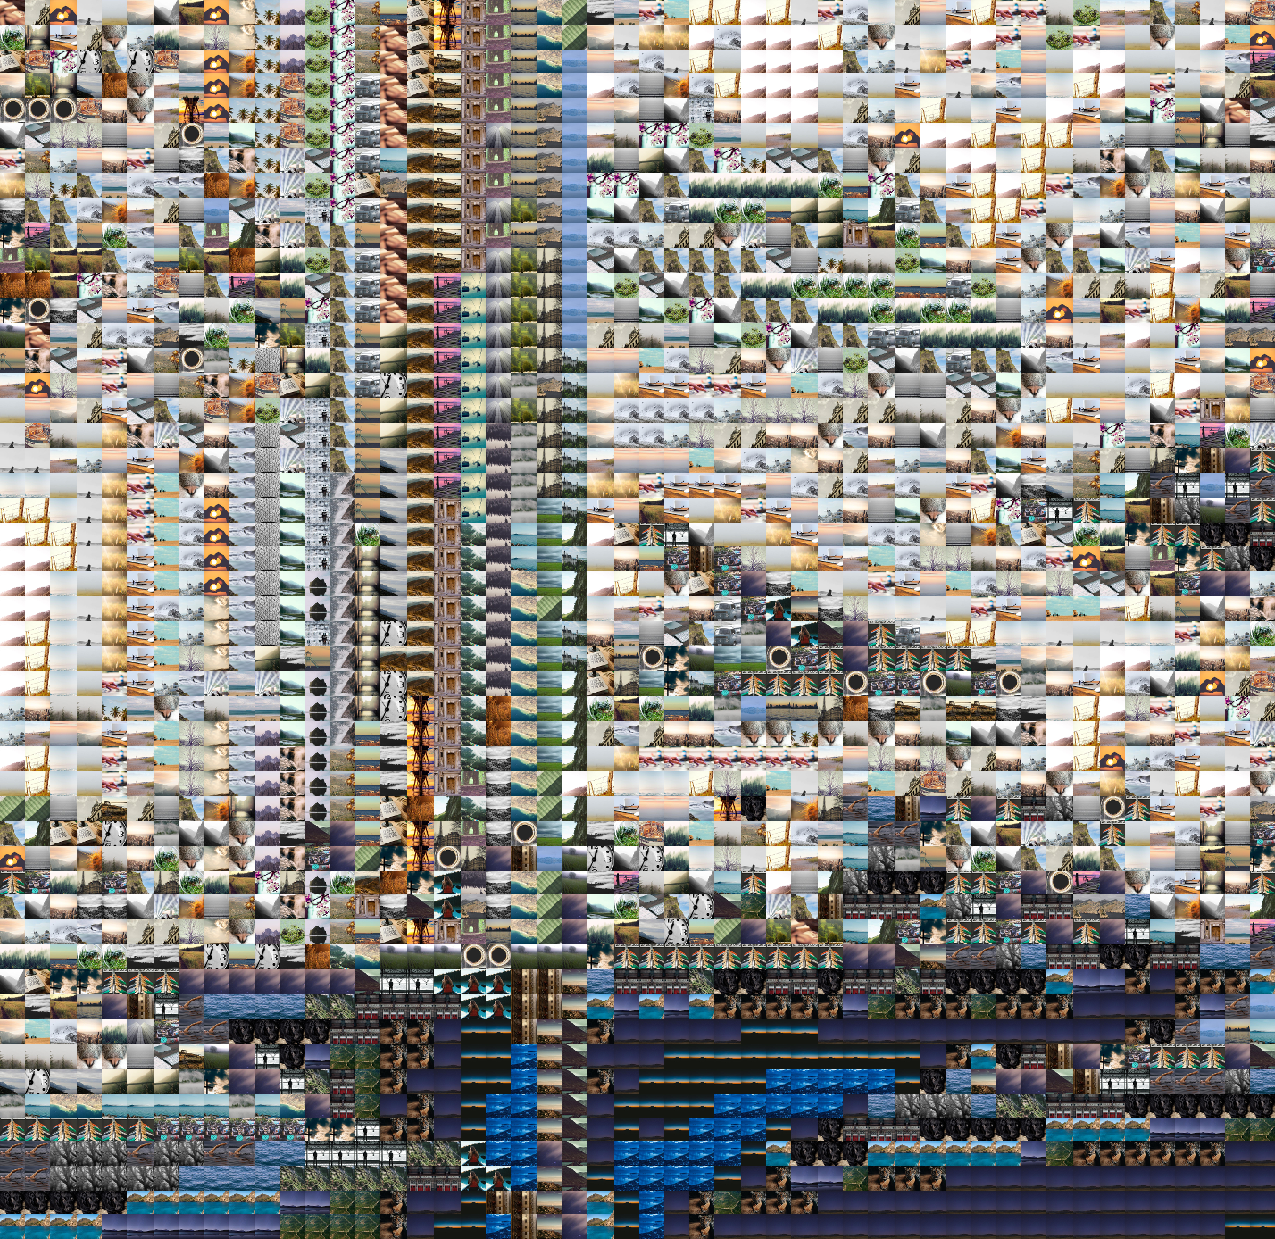
\includegraphics[height=5cm]{images/BadExample_Lines.pdf}
    }
    \subfloat[\centering mit mischung]{
        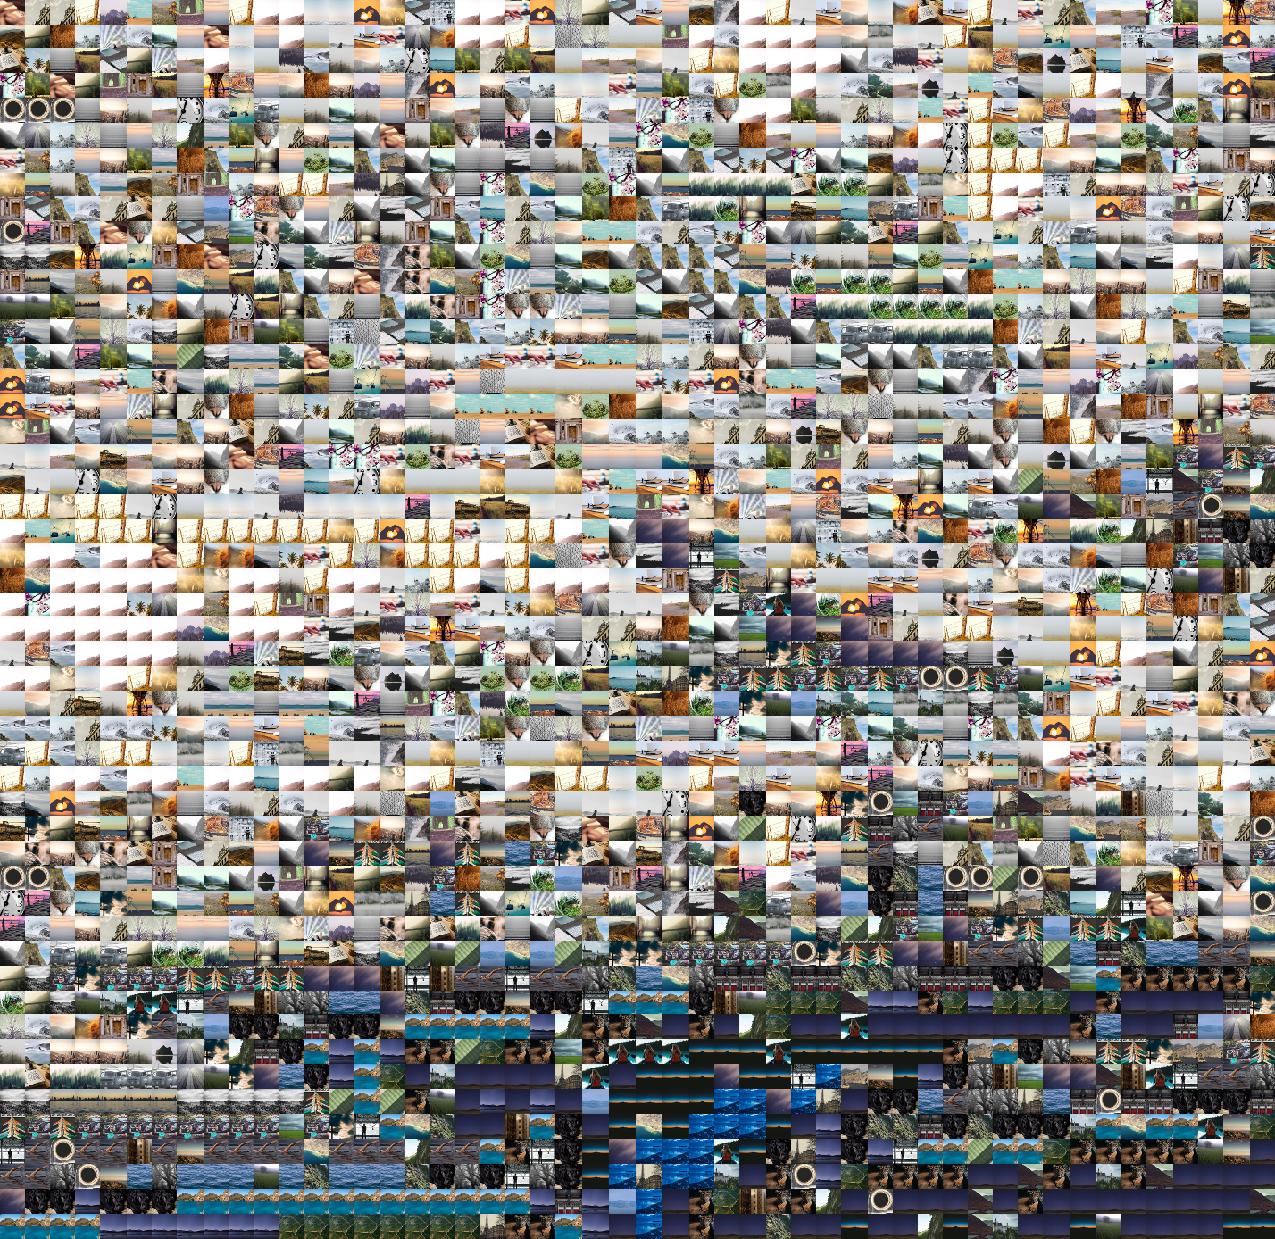
\includegraphics[height=5cm]{images/GodExample_NoLines.pdf}
    }
    \caption[Beste Bilder]{Unterschied zwischen mischen und nicht mischen}
\end{figure}

\begin{sloppypar}
Jeder ``Runnable'' sucht demnach nach dem besten Bild, welches noch verfügbar ist. Es werden dazu alle vorhandenen Datenbanken durchgegangen und für jede einzelne das beste Bild gesucht. Die besten aus alles Datenbanken werden dann verglichen und der beste wird gewählt. Um die beste Farbe einer Datenbank zu berechnen kann die java Methode ``Arrays.binarySearch'' verwendet werden. Diese Methode findet nicht nur den gleichen Wert, sondern auch einen index, an dem es den gesuchten Wert einsetzen würde. Anhand von dem Index wird dann im Array jeweils das nächste beste Bilde, welches noch nicht zu häufig verwendet wurde, gesucht. Die beiden gefundenen Werte, werden auf nähe zum gesuchten Wert überprüft. Der nähere wird dementsprechend auserwählt.
\end{sloppypar}

\newpage

\subsubsection{Skalieren der Bilder}
Das Skalieren der Bilder ist in drei Schritte einzuteilen. Das Management der Bilder, Berechnen der Zielgröße und das Skalieren an sich. Ich werde auf jeden Bereich individuell eingehen.

\paragraph{Management}\mbox{}\\
Da Ein Bild mehrfach ausgewählt werden kann, ist es wichtig ein Management System zu haben, welches verhindert, dass das selbe Bild nicht häufiger als nötig skaliert wird. Das Skalieren ist der Zeitaufwendigste Prozess, daher sollte dieser minimiert werden. Jedes Bild kann in vier unterschiedlichen Größen verwendet werden. Die Größen kommen aus dem in (siehe Berechnen der Sektionen) beschriebenen vorgehen. Werden die Bilder nur in einer einheitlichen Größe skaliert Entstehen schwarze Linien im Bild.

\begin{figure}[h]
    \centering
    \subfloat[\centering ohne mehrfach Skalierung]{
        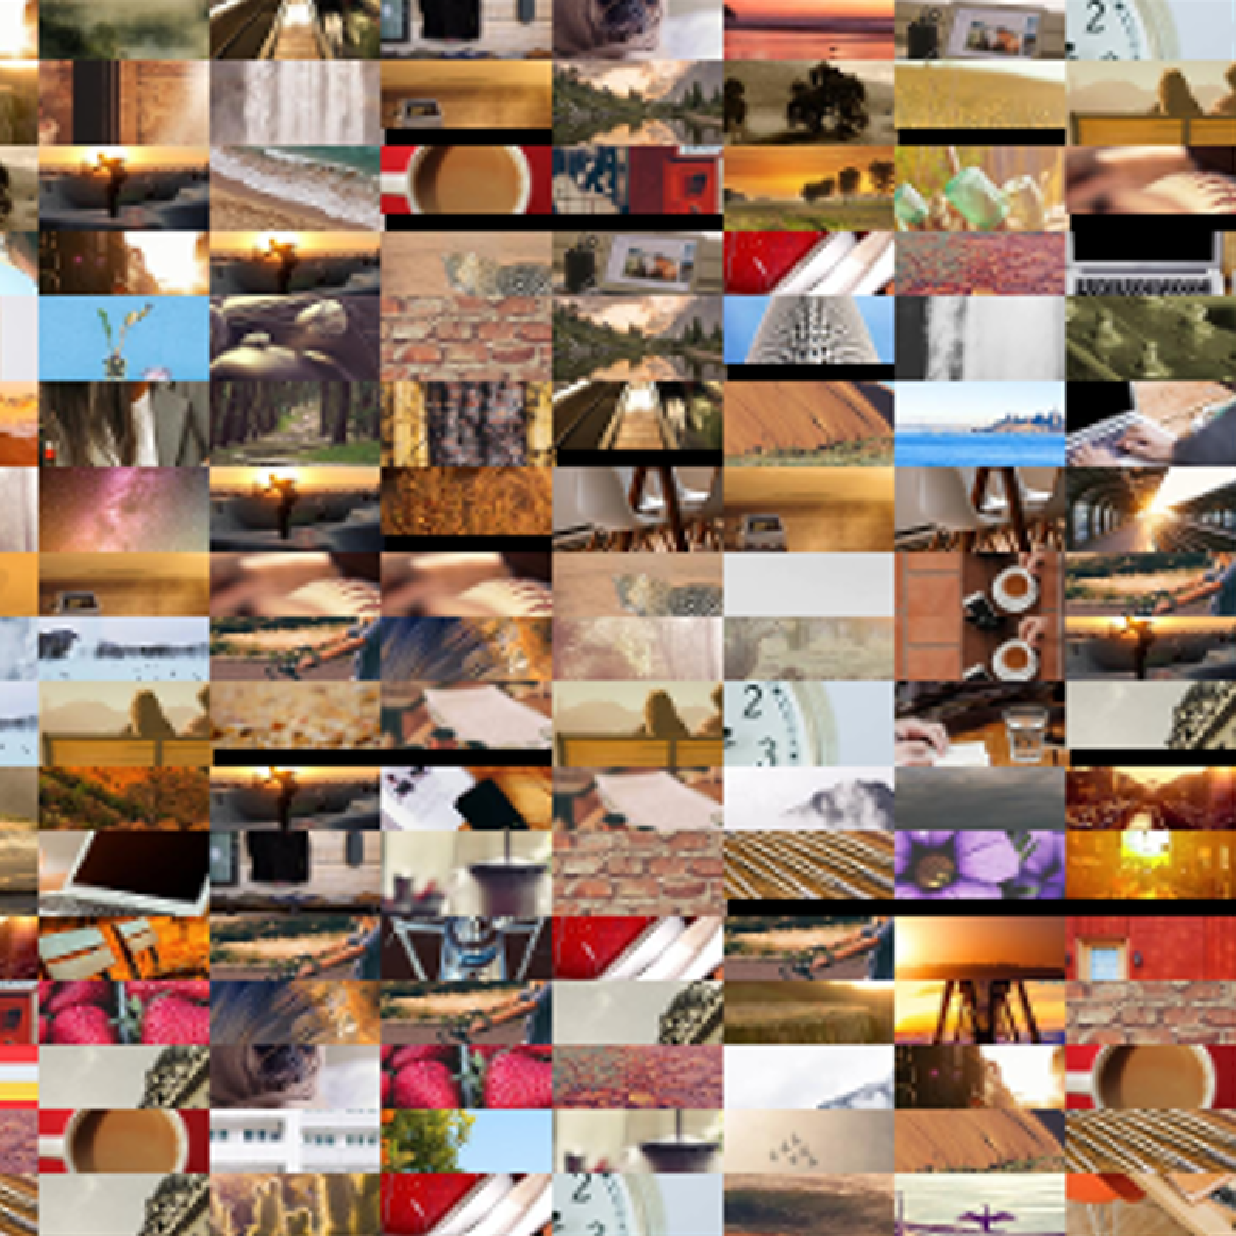
\includegraphics[height=5cm]{images/BadExample_BlackLines.pdf}
    }
    \subfloat[\centering mit mehrfach Skalierung]{
        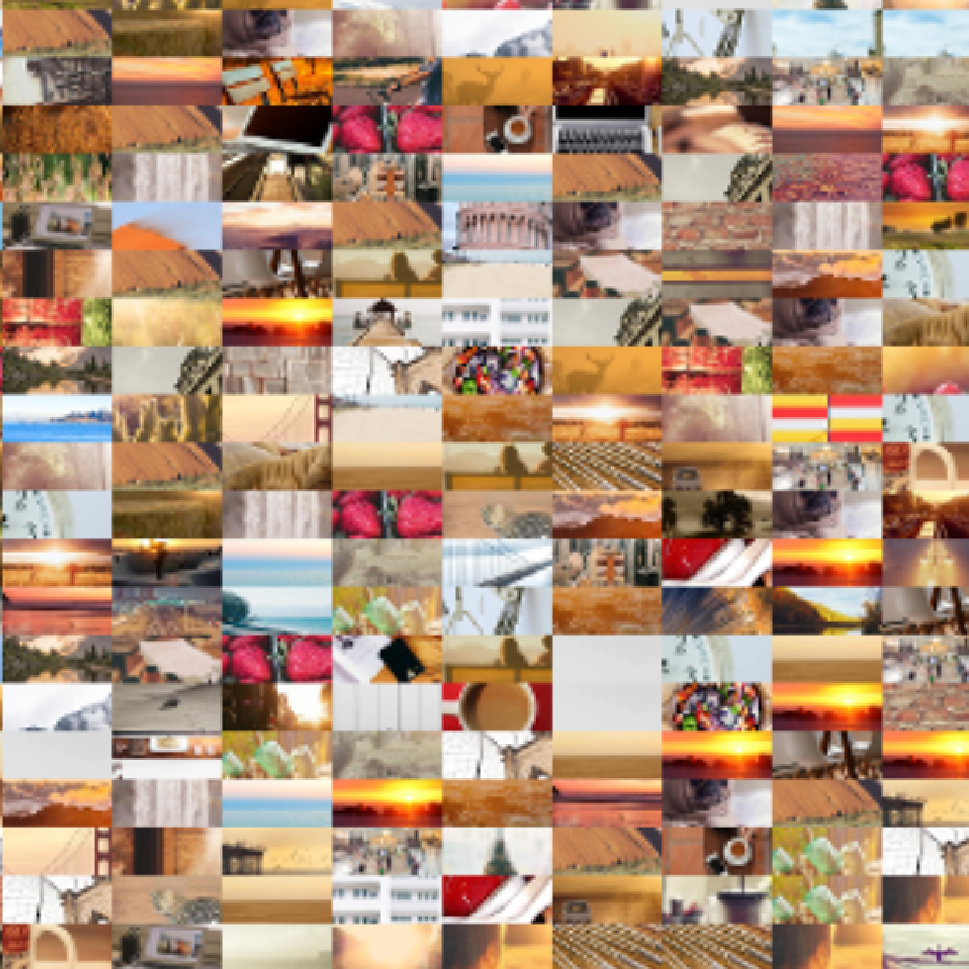
\includegraphics[height=5cm]{images/GodExample_NoBlackLines.pdf}
    }
    \caption[Schwarze Linien]{vierfache Skalierung der Bilder}
\end{figure}

Beim Managen wird demnach überprüft, ob ein bestimmtes Bild schon in der jeweiligen Größe vorhanden ist. Dazu wird eine Instanz der Klasse ``ScaledImages'' erzeugt. Diese Instanz fungiert als gemeinsamer Speicherort aller skalierten Bilder. Die Klasse hat ein zweidimensionales Array des Types ``ImageWithName'' und eine Methode ``exists()''. Die Methode ``exists()'' sucht mithilfe von dem Pfad des Bildes und den gewünschten Dimensionen in dem Array nach bereits skalierten Bildern. In dem Fall, dass etwas gefunden wird, werden die Koordinaten des gefunden Bildes zurückgegeben. Der Skalier-Thread speichert dan eine Referenz auf das gefundene Bild ab.
\medskip
\newline
Ein Problem beinhaltet das System jedoch noch. Es könnte zu der Situation kommen, dass mehrere Threads gleichzeitig mit dem gleichem Bildauftrag gestartet werden. Anfangs überprüft jeder Thread, ob sie arbeiten dürfen, oder das gewünschte Bild noch nicht existiert. Alle Threads werden davon ausgehen, dass die Arbeiten dürfen, da das Skalieren des Bildes und Speichern dessen vergleichsweise länger dauert als einen neuen Thread zu starten. Doch dadurch werden nicht nur Ressourcen unnütz verbraucht, sondern auch Fehler in der Bilddatei können entstehen, da mehrere Threads gleichzeitig eine Datei auslesen.

\begin{figure}[h]
    \centering
    \begin{minipage}{89mm}
        \fontsize{10pt}{11pt}\selectfont
        \def\svgwidth{8cm}
        \input{images/Manager_Threads.pdf_tex}
    \end{minipage}
    \begin{minipage}{1\textwidth-91mm}
        1. Überprüfen, ob die Bilder schon vorhanden sind.\\
        2. Schreiben des Bildes in das Array.
    \end{minipage}
    \caption[Thread und Manager]{Threads mit Manager}
\end{figure}

Um ein solches Verhalten zu verhindern, versucht ein Thread ein Bild zu reservieren, wenn es laut Manager frei ist. Ein Reserviertes Bild, wird als bereits existierendes gewertet. Das Referenz System funktioniert weiterhin, da keine neuen Objekte erstellt werden, sondern diese nur mit dem Bild befüllt werden. Die Array Struktur wird durch rasantes steigen des Speicherverbrauchs einzelner Objekte nicht beeinflusst. Das liegt unter anderem an dem ``GarbageCollector'' von Java, welcher auch in Stande is Arrays aus ihrem sonnst linearem Besetzen eines Speicherblockes im Arbeitsspeicher aufzuteilen, um unter anderem größer werdenden Objekten platz zu schaffen. Dabei werden interne Referenzen des Arrays überschrieben, um zu dem verschobenem Objekt zu zeigen.

\newpage

\paragraph{Berechnen der Zielgröße}\mbox{}\\
Das Ziel ist, die Bilder so gut wie möglich zu verwerten. Dazu müssen unterschiedliche Kriterien erfüllt werden. Erstens sollte das Bild nicht verzogen werden, zweitens sollte immer der größtmögliche Bereich des Bildes verwendet werden.

\begin{figure}[h]
    \centering
    \fontsize{12pt}{12pt}\selectfont% or whatever fontsize you like
    \def\svgwidth{12cm}
    \input{images/BerechnenZielgröße.pdf_tex}
    \caption[Berechnen Zielgröße]{Berechnen Zielgröße}
\end{figure}

Um das zu erreichen wird das Bild erst auf die Größe des gewünschten Sektors skaliert. Anschließend werden die Ränder abgeschnitten. Beim Skalieren wird versucht eine x-Achse des Bildes der y-Achse des Sektors anzupassen. Damit kann sichergestellt werden, dass das Bild seine Verhältnis beibehält. Wie in der oberen Grafik zu erkennen ist, wird ein Vertikal ausgerichtetes Bild in einen Horizontalen Sektor eingesetzt. Dazu wurde die x-Achse des Bildes auf die des Sektors skaliert. Die Formel zum Berechnen der y-Achse ist wie folgt.
\begin{align}
    y_\mathnormal{Bild\,neu}=y_\mathnormal{Bild\,alt} \cdot \frac{x_\mathnormal{sek.}}{x_\mathnormal{Bild\,alt}}
\end{align}    
Wenn die neu berechnete y-Achse kleiner ist als die des Sektors wird das selbe mit der x-Achse gemacht. Im letzten Schritt wird ein Abschnitt mittig aus dem skaliertem Bild mit den Abmaßen des Sektors geschnitten.

\newpage

\paragraph{Skalieren des Bildes}\mbox{}\\
Einleitend muss ich zu diesem Abschnitt sagen, dass ich die Folgenden Methoden nicht selber implementiert habe. Ich nutzte dazu die imgskalr library von Riyad Kalla, welche auf der Bilineare und Bikubischen Interpolation von Javas ``Graphics2D'' beruht.\cite{Scalr:Kalla} Im folgenden werde ich die Bilineare Interpolation erklären. Auf die Bikubische werde ich nur kurz eingehen.
\medskip
\newline
Bei dem Hochskalieren von Bildern stößt man auf das Problem, dass Farbwerte erfunden werden müssen. Andere Algorithmen erfinden keine neuen Farben und sind gut für Pixel Bilder geeignet. Für Landschaftsbilder würde dies lediglich ein verpixeltes Bild ergeben. Um neue Farbwerte zu Berechnen, wird bei der Bilinearen Interpolation linear Farbwerte berechnet.

\begin{figure}[h]
    \centering
    \subfloat[\centering Bilinear Start]{
        \tdplotsetmaincoords{65}{20}
    \begin{tikzpicture}[tdplot_main_coords, scale = 1.6]
        \filldraw[draw = black, fill = blue, opacity = 0.2](0,0,0) -- (3,0,0) -- (3, 3, 0) -- (0, 3, 0);

        \def \xy{{  {2, 1, 0.5, 1}, 
                    {4, 1, 2, 3}, 
                    {3, 2, 4, 1}, 
                    {0.5, 3, 5, 4}}}

        \foreach \x in {3,...,0}{
            \foreach \y in {3,...,0}{
                \draw[black](\x, 0, 0) -- (\x,3,0);
                \draw[black](0,\y,0) -- (3,\y,0);
            }
        }

        \foreach \x in {2,...,0}{
            \foreach \y in {2,...,0}{
                \pgfmathsetmacro\asInt{int(\xy[\y][\x])}
                \pgfmathsetmacro\r{(\asInt+1)/2}
                %bottom
                \filldraw[draw = black, fill = black, opacity = 0.05](\x,\y,0) -- (\x+1,\y,0) -- (\x+1,\y+1,0) -- (\x,\y+1,0);
                %top
                \filldraw[draw = black, fill = black, opacity = 0.15](\x,\y,\r) -- (\x+1,\y,\r) -- (\x+1,\y+1,\r) -- (\x,\y+1,\r);
                %front
                \filldraw[draw = black, fill = black, opacity = 0.05](\x,\y,0) -- (\x+1,\y,0) -- (\x+1,\y,\r) -- (\x,\y,\r);
                %back
                \filldraw[draw = black, fill = black, opacity = 0.075](\x,\y+1,0) -- (\x+1,\y+1,0) -- (\x+1,\y+1,\r) -- (\x,\y+1,\r);
                %rigth
                \filldraw[draw = black, fill = black, opacity = 0.1](\x+1,\y,0) -- (\x+1,\y+1,0) -- (\x+1,\y+1,\r) -- (\x+1,\y,\r);
                %left
                \filldraw[draw = black, fill = black, opacity = 0.125](\x,\y,0) -- (\x,\y+1,0) -- (\x,\y+1,\r) -- (\x,\y,\r);
            }
        }
        
        \foreach \xnum in {0,...,1}{
            \foreach \ynum in {0,...,1}{
                \node[draw] at (\xnum+0.5, \ynum+0.5) (a) {\xnum\,\ynum};
            }
        }

        \foreach \x in {2,...,0}{
            \foreach \y in {2,...,0}{
                \pgfmathsetmacro\asInt{int(\xy[\y][\x])}
                \pgfmathsetmacro\r{(\asInt+1)/2}
                
                \pgfmathsetmacro\nextx{\x==2 ? \x+0.5 : \x+1.5}
                \pgfmathsetmacro\nexty{\y==2 ? \y+0.5 : \y+1.5}

                \pgfmathsetmacro\nextXAsInt{int(\xy[int(\y)][int(\nextx)])}
                \pgfmathsetmacro\nextXr{(\nextXAsInt+1)/2}
                \pgfmathsetmacro\nextYAsInt{int(\xy[int(\nexty)][int(\x)])}
                \pgfmathsetmacro\nextYr{(\nextYAsInt+1)/2}
                \pgfmathsetmacro\nextXYAsInt{int(\xy[int(\nexty)][int(\nextx)])}
                \pgfmathsetmacro\nextXYr{(\nextXYAsInt+1)/2}

                \draw[thick, blue, -](\x+0.5,\y+0.5,0) -- (\x+0.5,\y+0.5,\r);
                \draw[fill = blue](\x+0.5,\y+0.5,\r) circle (2pt);
                \draw[thick, green, -](\x+0.5,\y+0.5,\r) -- (\nextx,\y+0.5,\nextXr);
                \draw[thick, green, -](\x+0.5,\y+0.5,\r) -- (\x+0.5,\nexty,\nextYr);
                
                \ifnum\x<2
                \ifnum\y<2
                    \pgfmathsetmacro\stepXY{1/3}
                    \pgfmathsetmacro\stepXXR{(\nextXr-\r)*\stepXY}
                    \pgfmathsetmacro\stepYYR{(\nextYr-\r)*\stepXY}
                    \pgfmathsetmacro\stepXYR{(\nextXYr-\nextYr)*\stepXY}
                    \pgfmathsetmacro\stepYXR{(\nextXYr-\nextXr)*\stepXY}
                    \foreach \xx in {0,...,1}{
                        \foreach \yy in {0,...,1}{
                            \pgfmathsetmacro\newX{\stepXY*(\xx+1)}
                            \pgfmathsetmacro\newY{\stepXY*(\yy+1)}
                            \pgfmathsetmacro\newXR{\r+\stepXXR*(\xx+1)}
                            \pgfmathsetmacro\newYR{\r+\stepYYR*(\yy+1)}
                            
                            \pgfmathsetmacro\nextYR{\nextYr+\stepXYR*(\xx+1)}
                            \pgfmathsetmacro\nextXR{\nextXr+\stepYXR*(\yy+1)}

                            \draw[thick, orange, -](\x+0.5+\newX,\y+0.5,\newXR) -- (\x+0.5+\newX,\y+1.5,\nextYR);
                            \draw[thick, orange, -](\x+0.5,\y+0.5+\newY,\newYR) -- (\x+1.5,\y+0.5+\newY,\nextXR);
                        }
                    }
                \fi
                \fi
            }
        }
        
    \end{tikzpicture}
    }
    \subfloat[\centering Bilinear Ende]{
        \tdplotsetmaincoords{50}{-15}
    \begin{tikzpicture}[tdplot_main_coords, scale = 1]
        \filldraw[draw = black, fill = blue, opacity = 0.2](0,0,0) -- (3,0,0) -- (3, 3, 0) -- (0, 3, 0);

        \def \xy{{  {2, 1, 0.5, 1}, 
                    {4, 1, 2, 3}, 
                    {3, 2, 4, 1}, 
                    {0.5, 3, 5, 4}}}

        \foreach \x in {0,...,3}{
            \foreach \y in {0,...,3}{
                \draw[fill = black](0,0,0) circle (2pt);
                \pgfmathsetmacro\asInt{int(\xy[\x][\y])}
                \pgfmathsetmacro\r{(\asInt+1)/2}
                \draw[black](\x, 0, 0) -- (\x,3,0);
                \draw[black](0,\y,0) -- (3,\y,0);
                %bottom
                \filldraw[draw = black, fill = red, opacity = 0.2](\x,\y,0) -- (\x+1,\y,0) -- (\x+1,\y+1,0) -- (\x,\y+1,0);
                %top
                \filldraw[draw = black, fill = red, opacity = 0.5](\x,\y,\r) -- (\x+1,\y,\r) -- (\x+1,\y+1,\r) -- (\x,\y+1,\r);
                %front
                \filldraw[draw = black, fill = red, opacity = 0.2](\x,\y,0) -- (\x+1,\y,0) -- (\x+1,\y,\r) -- (\x,\y,\r);
                %back
                \filldraw[draw = black, fill = red, opacity = 0.2](\x,\y+1,0) -- (\x+1,\y+1,0) -- (\x+1,\y+1,\r) -- (\x,\y+1,\r);
                %rigth
                \filldraw[draw = black, fill = red, opacity = 0.3](\x+1,\y,0) -- (\x+1,\y+1,0) -- (\x+1,\y+1,\r) -- (\x+1,\y,\r);
                %left
                \filldraw[draw = black, fill = red, opacity = 0.4](\x,\y,0) -- (\x,\y+1,0) -- (\x,\y+1,\r) -- (\x,\y,\r);
            }
        }
        \foreach \x in {0,...,2}{
            \foreach \y in {0,...,2}{
                \pgfmathsetmacro\asInt{int(\xy[\y][\x])}
                \pgfmathsetmacro\r{(\asInt+1)/2}
                
                \pgfmathsetmacro\nextx{\x==2 ? \x+0.5 : \x+1.5}
                \pgfmathsetmacro\nexty{\y==2 ? \y+0.5 : \y+1.5}

                \pgfmathsetmacro\nextXAsInt{int(\xy[int(\y)][int(\nextx)])}
                \pgfmathsetmacro\nextXr{(\nextXAsInt+1)/2}
                \pgfmathsetmacro\nextYAsInt{int(\xy[int(\nexty)][int(\x)])}
                \pgfmathsetmacro\nextYr{(\nextYAsInt+1)/2}
                \pgfmathsetmacro\nextXYAsInt{int(\xy[int(\nexty)][int(\nextx)])}
                \pgfmathsetmacro\nextXYr{(\nextXYAsInt+1)/2}

                \draw[thick, blue, -](\x+0.5,\y+0.5,0) -- (\x+0.5,\y+0.5,\r);
                \draw[fill = blue](\x+0.5,\y+0.5,\r) circle (2pt);
                \draw[thick, green, -](\x+0.5,\y+0.5,\r) -- (\nextx,\y+0.5,\nextXr);
                \draw[thick, green, -](\x+0.5,\y+0.5,\r) -- (\x+0.5,\nexty,\nextYr);
                
                \ifnum\x<2
                \ifnum\y<2
                    \pgfmathsetmacro\stepXY{1/2}
                    \pgfmathsetmacro\stepXXR{(\nextXr-\r)/2}
                    \pgfmathsetmacro\stepYYR{(\nextYr-\r)/2}
                    \pgfmathsetmacro\stepXYR{(\nextXYr-\nextYr)/2}
                    \pgfmathsetmacro\stepYXR{(\nextXYr-\nextXr)/2}
                    \foreach \xx in {0,...,0}{
                        \foreach \yy in {0,...,0}{
                            \pgfmathsetmacro\newX{\stepXY*(\xx+1)}
                            \pgfmathsetmacro\newY{\stepXY*(\yy+1)}
                            \pgfmathsetmacro\newXR{\r+\stepXXR*(\xx+1)}
                            \pgfmathsetmacro\newYR{\r+\stepYYR*(\yy+1)}
                            
                            \pgfmathsetmacro\nextYR{\nextYr+\stepXYR*(\xx+1)}
                            \pgfmathsetmacro\nextXR{\nextXr+\stepYXR*(\yy+1)}

                            \draw[thick, orange, -](\x+0.5+\newX,\y+0.5,\newXR) -- (\x+0.5+\newX,\y+1.5,\nextYR);
                            \draw[thick, orange, -](\x+0.5,\y+0.5+\newY,\newYR) -- (\x+1.5,\y+0.5+\newY,\nextXR);
                        }
                    }
                \fi
                \fi
            }
        }
    \end{tikzpicture}
    }
    \caption[Bilinear]{Bilineare Interpolation}
\end{figure}

Die unterschiedlichen Höhen in der der Grafik repräsentieren die Unterschiedlichen Farbwerte der Pixel. Das 3x3 Bild wird um den Faktor 3 skaliert. Zuerst wird ein Netz zwischen den einzelnen Werten gespannt. Die neuen Farbwerte entstehen an den Schnittpunkten des Netzes. Der Farbwert lässt sich somit mit den folgenden Gleichungen berechnen.
\begin{flalign}
    F_\mathnormal{neuX}=(F_\mathnormal{1\,0}-F_\mathnormal{0\,0})\cdot\frac{n_x}{S_\mathnormal{fak.}} \label{eq:WNeuX}\\
    F_\mathnormal{neuY}=(F_\mathnormal{1\,1}-F_\mathnormal{0\,1})\cdot\frac{n_y}{S_\mathnormal{fak.}} \label{eq:WNeuY}\\
    F_\mathnormal{neu}=F_\mathnormal{0\,0}+(F_\mathnormal{neuX})+(F_\mathnormal{neuY}-F_\mathnormal{neuX})\cdot\frac{n_y}{S_\mathnormal{fak.}} \label{eq:WNeu}
\end{flalign}
In den Gleichungen \ref{eq:WNeuX} und \ref{eq:WNeuY} werden die Start- und End-Punkte einer Netzlinie berechnet. $n_x$ und $n_y$ sind Zähler, welche die gewünschte Position in dem Teilnetz angibt. Das Maximum der beiden ist $S_\mathnormal{fak.}+1$. $S_\mathnormal{fak.}$ ist dabei der Faktor, um wie viel das Bild skaliert werden soll. Der Unterschied zischen Bilinearer Interpolation und Bikubischen ist, dass bei der Bilinearen lediglich zwei Linien aus jeweils zwei Punkte benutzt werden. Bei der Bikubischen werden vier kubische Spline Funktion aus jeweils vier Punkten benutzt. Der Vorteil der Bikubischen ist, dass das resultierende Bild einen höheren Kontrast bekommt. Auch können Komplexere Formen besser berücksichtigt werden.

\begin{figure}[h]
    \centering
    \subfloat[\centering Bilinear]{
        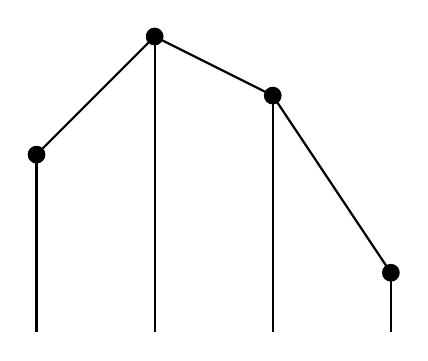
\begin{tikzpicture}[scale = 1.5]
    \def \valY{{2, 4, 3, 0.5}}

    \foreach \x in {0,...,3}{
        \pgfmathsetmacro\asInt{int(\valY[\x])}
        \pgfmathsetmacro\r{(\asInt+1)/2}
        \draw[thick, black, -](\x,0) -- (\x,\r);
        \draw[fill = black](\x,\r) circle (2pt);
        
        \pgfmathsetmacro\nextx{\x==3 ? \x : \x+1}
        \pgfmathsetmacro\nextAsInt{int(\valY[\nextx])}
        \pgfmathsetmacro\nextR{(\nextAsInt+1)/2}
        \draw[thick, black, -](\x,\r) -- (\nextx,\nextR);
    }
\end{tikzpicture}
    }
    \subfloat[\centering Bikubisch \protect\footnotemark]{
        %Berechnet mit https://tools.timodenk.com/cubic-spline-interpolation

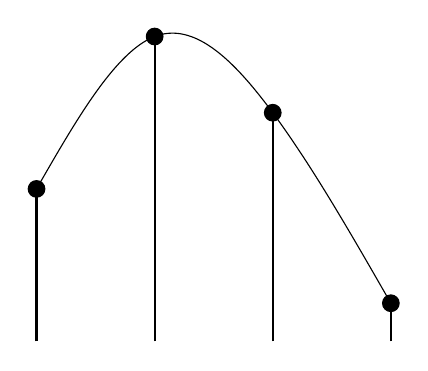
\begin{tikzpicture}[scale = 1.5]
    
        \pgfmathsetmacro\rEins{(+-0.7*0^3+1.32e-62*0^2+2.7*0^1+2*0^0)/1.55}
        \draw[thick, black, -](0,0) -- (0,\rEins);
        \draw[fill = black](0,\rEins) circle (2pt);

        \pgfmathsetmacro\rZwei{(+-0.7*1^3+1.32e-62*1^2+2.7*1^1+2*1^0)/1.55}
        \draw[thick, black, -](1,0) -- (1,\rZwei);
        \draw[fill = black](1,\rZwei) circle (2pt);

        \pgfmathsetmacro\rDrei{(+0.5*2^3+-3.6*2^2+6.3*2^1+0.8*2^0)/1.55}
        \draw[thick, black, -](2,0) -- (2,\rDrei);
        \draw[fill = black](2,\rDrei) circle (2pt);

        \pgfmathsetmacro\rVier{(+0.2*3^3+-1.8*3^2+2.7*3^1+3.2*3^0)/1.55}
        \draw[thick, black, -](3,0) -- (3,\rVier);
        \draw[fill = black](3,\rVier) circle (2pt);


    \draw[domain=0:1, smooth, variable=\x, black] plot ({\x}, {(+-0.7*\x^3+1.32e-62*\x^2+2.7*\x^1+2*\x^0)/1.55});
    \draw[domain=1:2, smooth, variable=\x, black] plot ({\x}, {(+0.5*\x^3+-3.6*\x^2+6.3*\x^1+0.8*\x^0)/1.55});
    \draw[domain=2:3, smooth, variable=\x, black] plot ({\x}, {(+0.2*\x^3+-1.8*\x^2+2.7*\x^1+3.2*\x^0)/1.55});
\end{tikzpicture}
    }
    \caption[BilinearBikubisch]{Vergleich Bilinear und Bikubisch}
\end{figure}
\footnotetext{Funktion mit \url{https://tools.timodenk.com/cubic-spline-interpolation} erstellt}

\medskip
Um die beste Qualität dei dem Runterskalieren zu erhalten, wird das Bild häufiger skaliert. Dies verwaltet die imgskalr library. Das Bild wird wiederholt um $\frac{1}{7}$ seiner Breite und Höhe verkleinert. Der Wert wurde nicht Mathematisch berechnet, sondern wurde durch testen herausgefunden.\cite{Scalr:Kalla}

\begin{figure}[h]
    \centering
    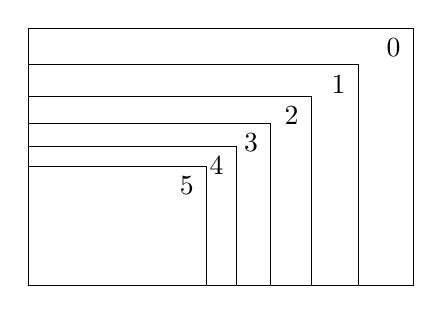
\begin{tikzpicture}[scale = 0.1]
    \def \xy {{{4890,3263},
               {4192,2797},
               {3594,2398},
               {3081,2056},
               {2641,1763},
               {2264,1512}}}

    \foreach \x in {0,...,5}{
        \pgfmathsetmacro\width{int(\xy[\x][0])/100}
        \pgfmathsetmacro\height{int(\xy[\x][1])/100}
        \draw[black](0,0)--(\width,0)--(\width,\height)--(0,\height)--(0,0);
        \node[] at (\width-2.5,\height-2.5) (a) {\x};
    }

\end{tikzpicture}
    \caption[Inkrementell]{Inkrementelles Skalieren}
\end{figure}
\newpage

%Die Laufzeitanalyse
\section{Laufzeitanalyse}
\subsection{Einleitung}
Um die Effizienz des Programms beurteilen zu können, werde ich die einzelnen Algorithmen betrachten. Dazu werde ich Das erstellen einer Datenbank, berechnen der durchschnittlichen Farbe, skalieren der Bilder und das berechnen der besten Bilder vergleichen. Der Test kann mit einer UI im Programm durchgeführt werden. Es wird ein Test mehrfach durchgeführt und bei jedem neuem Durchgang die Anzahl an Bildern erhöht. Das Testen kann mit generierten Bildern und mit zufälligen Bildern der Internetseite ``https://picsum.photos'' durchgeführt werden. Alle folgenden Tests werden mit zufälligen Bildern durchgeführt, da diese die echte Benutzung am besten Simulieren. Bei den Generierten Bildern sinken die Berechnungszeiten stark, da weniger Farbkomplexität gegeben ist. Bei jeder Simulation wird auch der benötigte Arbeitsspeicher gespeichert, da das Programm sehr Arbeitsspeicher intensiv werden kann. Die Laufzeit des Berechnen der durchschnittlichen Farbe, das erstellen einer Datenbank und das berechnen der besten Bilder ist Linear. $O(n)$ mit der Anzahl der Bilder als $n$. Die Laufzeit des Skalieren ist abhängig von dem genutzten Algorithmus.
\begin{figure}[h]
    \centering
    \subfloat[\centering Datenbank]{
        \begin{tikzpicture}[scale = 0.85]
            \begin{axis}[tick label style={
                /pgf/number format/fixed,
                /pgf/number format/fixed zerofill,
                /pgf/number format/precision=1
            }, legend pos=north west, no markers, legend style={nodes={scale=0.7, transform shape}}]
                \addplot table [x=x, y=time, col sep=semicolon] {./images/Simulationen/Database_1.000x10.000.csv};
                \addlegendentry{Zeit in ns}
                \addplot table [x=x, y=ram, col sep=semicolon] {./images/Simulationen/Database_1.000x10.000.csv};
                \addlegendentry{Ram in Byte}
            \end{axis}
        \end{tikzpicture}
        \label{DatenbankGraph}
    }
    \subfloat[\centering durchschnittliche Farbe]{
        \begin{tikzpicture}[scale = 0.85]
            \begin{axis}[tick label style={
                /pgf/number format/fixed,
                /pgf/number format/fixed zerofill,
                /pgf/number format/precision=1
            }, legend pos=north west, no markers, legend style={nodes={scale=0.7, transform shape}}]
                \addplot table [x=x, y=time, col sep=semicolon] {./images/Simulationen/averageColor_500x50_500x500_Ultra.csv};
                \addlegendentry{Zeit in ns}
                \addplot table [x=x, y=ram, col sep=semicolon] {./images/Simulationen/averageColor_500x50_500x500_Ultra.csv};
                \addlegendentry{Ram in Byte}
            \end{axis}
        \end{tikzpicture}
        \label{DurchschnittlicheFarbeGraph}
    }
    \hspace{0mm}
    \subfloat[\centering skalieren der Bilder]{
        \begin{tikzpicture}[scale = 0.85]
            \begin{axis}[tick label style={
                /pgf/number format/fixed,
                /pgf/number format/fixed zerofill,
                /pgf/number format/precision=1
            }, legend pos=north west, no markers, legend style={nodes={scale=0.7, transform shape}}]
                \addplot table [x=x, y=time, col sep=semicolon] {./images/Simulationen/scalingImages.csv};
                \addlegendentry{Bilinear(ns)}
                \addplot table [x=x, y=time, col sep=semicolon] {./images/Simulationen/scalingImagesBikubisch.csv};
                \addlegendentry{Bikubisch(ns)}
                \addplot table [x=x, y=ram, col sep=semicolon] {./images/Simulationen/scalingImages.csv};
                \addlegendentry{Bilinear(Byte)}
                \addplot table [x=x, y=ram, col sep=semicolon] {./images/Simulationen/scalingImagesBikubisch.csv};
                \addlegendentry{Bikubisch(Byte)}
            \end{axis}
        \end{tikzpicture}
        \label{SkalierenGraph}
    }
    \subfloat[\centering berechnen der besten Bilder]{
        \begin{tikzpicture}[scale = 0.85]
            \begin{axis}[tick label style={
                /pgf/number format/fixed,
                /pgf/number format/fixed zerofill,
                /pgf/number format/precision=1
            }, legend pos=north west, no markers, legend style={nodes={scale=0.7, transform shape}}]
                \addplot table [x=x, y=time, col sep=semicolon] {./images/Simulationen/computation.csv};
                \addlegendentry{Zeit in ns}
                \addplot table [x=x, y=ram, col sep=semicolon] {./images/Simulationen/computation.csv};
                \addlegendentry{Ram in Byte}
            \end{axis}
        \end{tikzpicture}
        \label{BesteBilderGraph}
    }
    
    \caption[BilinearBikubisch]{Vergleich Bilinear und Bikubisch}
\end{figure}
Test \ref{DatenbankGraph} wurde von $10000$ bis $10000000$ Bilder durchgeführt. Die Zeit erhöht sich um 1250ns pro Bild. Die Arbeitsspeichernutzung erhöht sich um 87Byte pro Bild. Die Arbeitsspeichernutzung ist dabei auch stark von der Länge des Speicherortes des Bildes abhängig.
\newline
Test \ref{DurchschnittlicheFarbeGraph} wurde von $1000$ bis $25000$ Bilder durchegführt. Die Bilder hatten eine größe von 500x500px. Die Laufzeit für ein Bild liegt bei 1,09ms. Für jedes weitere Bild werden 88kByte verbraucht. Beide Werte verhalten sicht linear zu der Anzahl der Bilder.
\newline

ÜBERPRÜFEN!!!!

Das Skalieren der Bilder in \ref{SkalierenGraph} wurde jeweils mit einem Bilinearen Algorithmus und einem Bikubischen Algorithmus durchgeführt. Dazu wurden 500x500px große Bilder auf 100x70px scaliert. Der Test wurde mit $1000$ Bildern gestartet und mit $12500$ beendet. Es ist zu erkennen, dass nur ein geringer Laufzeitunterschied von $\Delta t = 4,2ms - 3,7ms = 0,5ms$ zwischen den beiden Algorithmen besteht. Dieser geringe unterschied kommt daher, dass beide Algorithmen sich sehr ähnlich verhalten. Der Unterscheid liegt lediglich bei der komplexeren Berechnung in dem Bikubischem Algorithmus, welche nur einen Teil der Laufzeit beansprucht.
\newpage

%Schluss
\section{Schluss}
Das Bearbeiten dieser Arbeit hat mich vieles gelehrt. Nicht nur habe ich ein tieferes Verständnis für das Programmieren bekommen, sondern auch das Managen von großen Projekten\footnote{Das Projekt betrug über 5540 Zeilen Code in 49 Klassen.}. Jedoch war der ``Do it yourself'' Weg nicht immer leicht und es war nicht immer einfach etwas richtiges zu finden. Besonders weil das Thema Prozesse nicht das Bekannteste im Internet ist. Meine Anfangs naive Einstellung ``Threads sind nur da um mehr Kerne zu nutzen.'' hat sich als Falsch herausgestellt. Die Enorme Komplexität hinter den wohl wichtigsten Prinzipien für die Moderne Welt ist nicht zu überschätzen. Ich habe mich schließlich im Linux Kernel Code wiedergefunden um zu verstehen, wie ein \textit{Scheduler} funktioniert.

\subsection{Aussicht}
In meinen Zukünftigen Projekten möchte ich meine Nutzung von Threads weiterhin verbessern. Aber auch möchte ich noch mehr Funktionen zu meinem Programm hinzufügen. Ein weiterer Meilenstein, den ich mir erarbeiten möchte ist die Nutzung der Grafikkarte. Die Enormen Rechenkapazitäten, welche in der Grafikkarte verborgen ist, würde mir neue Türen für noch größere Projekte öffnen.
\newpage

%Literaturverzeichnis
\bibliographystyle{gerabbrv}
\bibliography{src/literatur}
\end{document}